\section{Lokale Extrema unter Nebenbedingungen}
Sei $f:D\rightarrow \R, D\subseteq \R^n$ offen. Wir wollen diese Funktion maximieren oder minimieren, allerdings nicht auf dem ganzen Definitionsbereich, sondern unter einer Nebenbedingung. Das heißt innerhalb von $D$ ist eine Teilmenge durch eine Gleichung festgelegt, d.h. es gibt eine Funktion $g:D\rightarrow \R$. Gesucht sind alle Punkte $x\in D$, die $f$ z.B. maximieren unter der Nebenbedingung $g(x)=0$. Wir wollen dabei annehmen, dass $\nabla g(x)\neq 0$ für alle $x\in D$.

\paragraph{Geometrische Überlegung}
Ist $c:(-\epsilon,\epsilon)\rightarrow D$ eine Kurve, so dass $f\circ c(t)$ bei $t=t_0$ ein lokales Extremum annimt: Dann gilt nach Kettenregel
\begin{align*}
	0&=\left(f\circ c\right)'(t_0)\\
	&=Df(\underbrace{c(t_0)}_{=x_0}) *\dot c(t_0)\\
	&=\nabla f(x_0)*\dot c(t_0)
\end{align*}
(Wobei hier das Skalarprodukt verwendet wird.)
Die Ableitungsvektoren aller solcher Kurven durch den Punkt $x_0$ mit $c(t_0)=x_0$ müssen also bei $t_0$ senkrecht auf $\nabla f(x_0)$ stehen. Andererseits steht der Gradient $\nabla g$ senkrecht auf den Niveaumengen von $g$, also gilt bei $x_0$
\begin{equation*}
	\nabla f(x_0)=\lambda \nabla g(x_0)
\end{equation*}
das heißt die Gradienten von $f$ und $g$ sind bei $x_0$ parallel. Die reelle Konstante $\lambda$ heißt \emph{Lagrange-Multiplikator}.

\paragraph{Beispiel:} (aus der Volkswirtschaftslehre) Für positive $x_1,\ldots,x_n$ sei durch
\begin{equation*}
	f(x_1,\ldots,x_n) =ax_1^{\alpha_1}\ldots x_n^{\alpha_n}
\end{equation*}
mit $a,\alpha_i>0$ eine Cobb-Douglas-Funktion gegeben. Dies ist zum Beispiel eine
\begin{itemize}
	\item Produktionsfunktion, $x_i$ die Inputs
	\item Nutzenfunktion, wobei $x_i$ die von einem Verbraucher konsumierten Güter sind.
\end{itemize}
Auf $(0,\infty)^n$ hat die Funktion eine Maxima oder Minima, aber unter einer Nebenbedingung, z.B. einer Budgetbeschränkung, kann es lokale Maxima unter diesen Einschränkungen geben. Z.B.
\begin{equation*}
	g(x)=p_1 x_1+\ldots+p_nx_n-b
\end{equation*}
mit $p_i$ den Preisen und $b$ dem Budget.

\paragraph{Beispiel:}
Für $n=2, f(x,y)=x^{\sfrac 12}*y^{\sfrac 12}=\sqrt{x*y}$ sei die Nutzenfunktion und sei durch $x+2y=1$ eine Budgetbeschränkung gegeben, d.h. $g(x,y)=x+2y-1$. Wir suchen lokale Extrema von $f$ unter der Nebenbedingung $g=0$. Dazu
\begin{equation*}
	\nabla f(x,y)=\vector{\frac 12 x^{\sfrac {-1}2}*y^{\sfrac 12}\\
	\frac 12 x^{\sfrac 12}*y^{\sfrac {-1}2}
	}
\end{equation*}
und \begin{equation*}
	\nabla g(x,y)=\vector{1\\2}
\end{equation*}
Der Ansatz $\nabla f(x,y)=\lambda\nabla g(x,y)$ führt zu
\begin{equation*}
	\vector{\frac 12 x^{\sfrac {-1}2}*y^{\sfrac 12}\\
	\frac 12 x^{\sfrac 12}*y^{\sfrac {-1}2}} =
	\vector{\lambda\\2\lambda}
\end{equation*}
d.h. auf die Gleichungen
\begin{align*}
	\frac 12 x^{\sfrac {-1}2}*y^{\sfrac 12}&=\lambda\\
	\frac 12 x^{\sfrac 12}*y^{\sfrac {-1}2}&=2\lambda
\end{align*}
Die Existenz eines $\lambda\in\R$ so dass beide Gleichungen erfüllt sind, ist äquivalent zu
\begin{equation*}
	2x^{\sfrac {-1}2}*y^{\sfrac 12}=x^{\sfrac 12}*y^{\sfrac {-1}2}\enspace\Leftrightarrow\enspace
	2y=x
\end{equation*}
Zusammen mit der Nebenbedingung $x+2y=1$ erhalten wir als einzige lokalen Flachpunkt unter Nebenbedingungen den Punkt $(x,y)=\left(\frac 12, \frac 14 \right)$.

\begin{center}
	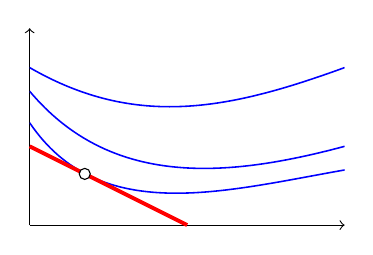
\begin{tikzpicture}
		\draw[black, ->] (0,0) to (4,0);
		\draw[black, ->] (0,0) to (0,2.5);

		\begin{scope}
			\clip (0,0) rectangle (4,2.5);

			\draw[blue, line width=0.2mm] (0,1.3) to[out=-56,in=190] (4,0.7);
			\draw[blue, line width=0.2mm] (0,1.7) to[out=-50,in=195] (4,1);
			\draw[blue, line width=0.2mm] (0,2) to[out=-30,in=200] (4,2);
		\end{scope}

		\draw[red, line width=0.5mm] (0,1) -- (2,0);

		\draw (0.7,0.65) node [fill = white,circle,inner sep = 0pt,minimum size = 4pt,draw] {};
	\end{tikzpicture}
\end{center}

\paragraph{Bemerkungen:}
\begin{enumerate}
	\item Die Lagrangemultiplikatorbedingung $\nabla f(x)=\lambda \nabla g(x)$ ist nur eine notwendige Bedingung für ein lokales Extremum. Für eine hinreichende siehe Sändig-Skript.
	\item Bei der obigen Aufgabe kann man das Extremum auch finden, indem man die Menge $\set{(x,y)\in D}{g(x,y)=0}$ durch die Abbildung
	\begin{equation*}
		l:t\mapsto \vector{t\\\frac{1-t}2}, [0,1]\rightarrow \R^2
	\end{equation*}
	parametrisiert, die sogenannte \emph{Substitutionsmethode}. Man betrachte dazu die Funktion $f\circ l(t)$.
\end{enumerate}
